% !TeX encoding = UTF-8
% !TeX program = pdflatex
% !BIB program = biber

%%% To write an article in English, please use the option ``english'' in order
%%% to get the correct hyphenation patterns and terms.
%%% \documentclass[english]{class}
%%% for anonymizing an article you can use the ``anonymous'' option.
%%%
%%% Um einen Artikel auf deutsch zu schreiben, genügt es die Klasse ohne
%%% Parameter zu laden.
%%% Zur Anonymisierung kann die ``anonymous'' Option genutzt werden.
\documentclass[english]{lni}
\usepackage{dirtytalk}
\usepackage{graphicx}

\addbibresource{sources.bib} 


%%
\begin{document}
%%% Mehrere Autoren werden durch \and voneinander getrennt.
%%% Die Fußnote enthält die Adresse sowie eine E-Mail-Adresse.
%%% Das optionale Argument (sofern angegeben) wird für die Kopfzeile verwendet.
\title[Ein Kurztitel]{Exposé for the Master's Thesis \textit{Augmenting Enterprise Architecture Landscapes with AI: A Retrieval-Augmented Chatbot Approach using Graph Databases}}
%% \subtitle{Untertitel / Subtitle} % if needed
 \author[1]{Hendrik Gruber}{hendrik.gruber@stud.fra-uas.de}{}
 \affil[1]{Frankfurt University of Applied Sciences}
\maketitle

%\begin{abstract}
%Dies ist eine kurze Übersicht über das Dokument mit einer Länge von
%70 bis 150 Wörtern. Es sollte ein Absatz sein, der die relevantesten
%Aspekte enthält.
%\end{abstract}


This exposé outlines what, why, and how the work for my planned master's thesis will be conducted. The goal of this exposé is to provide an overview of the subject matter and to demonstrate my understanding of the research topic.

\begin{keywords}
AI chatbot, Retrieval-Augmented Generation (RAG), Enterprise Architecture Management (EAM), Graph Database.
\end{keywords}
%%% Beginn des Artikeltexts
%\section{Überschrift/Heading}


\section{Problem Statement and Research Questions}
Within the realm of Enterprise Architecture Management (EAM), updating and maintaining the architecture landscape and documentation when new projects or applications arise can be a tedious task. It requires that the Enterprise Architect (EA) understands the existing application landscape and the changes required to reflect these new incoming initiatives in a way that preserves consistency, avoids redundancies in the landscape, and while also supporting the organization's strategic goals. Because the landscape of a company can be highly complex, containing hundreds of applications, projects, and connections between them, seeing the big picture can be a difficult task for an individual or even for an entire team \cite{jung2021masterclass}. This task can be slow and error prone.

This is a laborious task which can potentially be supported with the help of generative AI \cite{ramachandran2025transforming}. AI can read in application landscape diagrams and project descriptions written in natural language and embed these into a graph database allowing an EA to retrieve information via chat. However, as it stands, there is a lack of generative AI solutions for this specific problem. All publicly existing solutions found are only theoretical work.

The master's thesis will be taking on the following research question: \say{\textbf{How can generative AI support Enterprise Architects in assessing and documenting the effects of new or changing projects in the application landscape?}} Three supplementary questions will be answered when approaching the main thesis question:
\begin{enumerate}
    \item \say{What are the current challenges faced by Enterprise Architects when updating landscapes and documenting changes when new projects occur?}
    \item \say{How can application landscapes and project descriptions be transformed into graph-based representations that reflect the existing landscapes?}
    \item \say{How effective is a generative AI chatbot in supporting Enterprise Architects?}
\end{enumerate}


\section{Literature and State of the Art}
The following literature research was conducted as a preliminary search in order to understand the gap my thesis could fill. Google Scholar was primarily used as well as academic sources after 2022, especially for sources regarding chatbots and AI. ChatGPT's deep research feature was also used as a supplement research method after describing to it what my thesis' subject is about. This list of literature is not exhaustive and further research will be conducted for the final thesis. The sources are clustered and briefly described as follows.

\subsection{Enterprise Architecture Management}
The 2021 book from Jung and Fraunholz \cite{jung2021masterclass} goes into detail on how EAM works, what challenges EAs face during their tasks, and gives a foundation to build upon when analyzing how to improve the process of documenting changes. Especially chapter 5 will give a scientific basis for everything regarding EAM and EAs.

\subsection{Human-Chatbot-Interaction}
The 2025 paper from Ramachandran \cite{ramachandran2025transforming} focuses on how software architects can leverage chatbots such as ChatGPT to aid in creating software diagrams such as Unified Modeling Language (UML) diagrams. The paper notes limitations when creating actual diagrams. They were often inconsistent and less robust than the human-created version. Some chatbots were also very sensitive to the input prompts. This is relevant for my thesis as the EAM chatbot will also be generating an output that may be susceptible to these shortcomings and knowing potential errors beforehand will be helpful during development.

\subsection{Graph Databases and Graph Embeddings}
The 2023 paper from Besta et al. \cite{besta2023demystifying} gives a solid foundation on how graph databases work. It covers how they organize data, how they are designed, and what types of queries a graph database can support. This paper will deem useful to understand and describe the basic functionality of graph databases.

Taking complex data such as the landscape diagrams and project descriptions and embedding these in a graph database in a way that represents the data correctly will be one of the main challenges during the implementation phase. The 2020 paper from Grohe \cite{grohe2020word2vec} describes that the quality of the vector representations is decisive for usefulness of the data. This paper gives an overview of different embedding methods such as word2vec and methods to understand the embeddings.

\subsection{Large Language Models and Retrieval-Augmented Generation}
The 2024 paper by Zhao et al. \cite{zhao2024retrieval} describes how RAG works and how it supplements Large Language Models (LLMs) in order to allow domain-specific answers. It also describes the challenges of retrieving the augmented data, accurately interpreting the user's intent, and fully harnessing the capabilities of the LLM.

What stands out is that there are limited publicly documented implementations of an RAG-based AI chatbot which helps EAs with their workload when documenting a changing landscape. This is the literary gap that my thesis will attempt to fill. The above literature will be used to give the reader of my thesis the necessary understanding of the subject matter before diving into my methodology.

\section{Methodology and Approach}
Conducting this research will require a prototype-driven approach. An AI chatbot will be developed which can interact with an EA. The chatbot will be trained with real-world data and will be able to augment its generated responses by accessing this data in a graph database. The EA will be able to use natural language within a chat prompt, similar to the user interface of existing chatbots such as ChatGPT. It will be able to hold a conversation with the EA about the planned changes and effects within the realm of the provided data and landscape architecture.

\subsection{System Architecture}
The architecture of the prototype will consist of five basic elements, as shown in figure \ref{fig:arch_diagram}. The provided data, which contains project and application factsheets, will be vectorized and read into a graph database. Once the data is stored in the database, the LLM is able to retrieve data from it and augment its response with the real-world project data. An out-of-the-box LLM will be used in this case and no new LLM will be trained.

The EA will then be granted access to a web application containing a chat UI. The EA may ask questions such as "For project x, I need to be able to document requirements and manage progress on tasks. I need new software for this and need to understand how my application landscape will be affected by this and how to document it." The chatbot will be able to ask for more information and get everything it needs from the EA to be able to answer the given prompt. It then makes a suggestion on what the EA can do and and updates the documentation and landscape accordingly. The LLM will be prompted to stick to the topic of EAM and is able to hold a conversation on the subject matter.

\subsection{Anticipated Challenges}
Implementing this prototype will come with its own challenges as it contains complex requirements. One foreseeable challenge will be converting the provided data into vectors, nodes, and edges and inserting it into the graph database in such a way that the data can later be augmented in realtime. Many different methods exist to embed data into vectors, nodes, and edges and finding a method that represents the project and application landscape in a useful way is a hurdle that needs to be overcome.\cite{grohe2020word2vec}

Another challenge may be heterogeneous data formats or generally inconsistent data. The format of the factsheets may be different or have different data types. Some project's or application's factsheets may also have varying depths of information. E.g. one project may be described in detail while another project may only be described at surface level.

The effects of data complexity and the corresponding risk of latency is currently not known. If there are hundreds of application and project descriptions which will be embedded into the vector database, then applying RAG on large scale graph database could potentially cause latency in response times.

\begin{figure}[h]
\centering
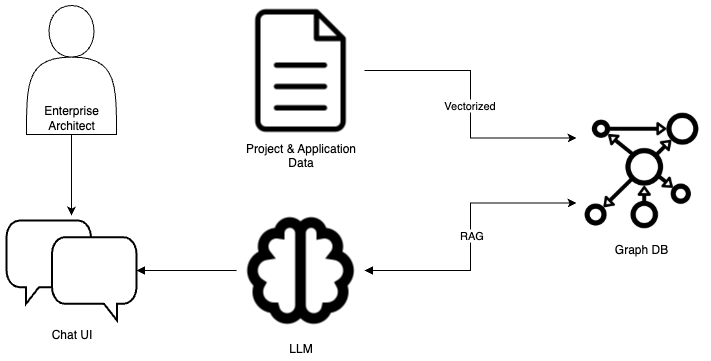
\includegraphics[scale=0.5]{./architecture_diagram.png}
\caption{A first draft architecture diagram of the expected system components and points of interaction between them.}
\label{fig:arch_diagram}
\end{figure}

\section{Expected Contribution}
The contribution of this thesis is to propose a scientifically sound methodology for building an LLM-based chatbot in the realm of EAM. The work will identify strengths, limitations, and challenges of combining graph-based knowledge with retrieval-augmented generation, and will derive design principles and evaluation criteria for such systems. Furthermore, the thesis will provide guidance on how to critically assess embedding quality, retrieval effectiveness, and the trade-offs involved in integrating structured and unstructured data. In doing so, it contributes both practical insights for enterprise architects and a foundation for future research on AI-assisted EAM tools.

The deliverables of my thesis will include the following:
\begin{itemize}
	\item Prototype implementation
	\item Reference metamodel which defines a schema that maps the given project documentation into a graph structure usable for retrieval
	\item Evaluation toolkit consisting of prompts that can be asked, metrics on how to measure the performance of the chatbot, and a rubric on how to rate the results
	\item Design principles and lessons learned
\end{itemize}

\section{Thesis Outline and Structure}
The following general structure will be followed for the thesis:

\begin{itemize}
    \item Introduction, Motivation, and Thesis Question
    \item Background Information (Foundational Concepts such as EAM, LLMs, RAG, Graph DBs)
    \item Current State of the Art and Literature
    \item Methodology and System Design
    \item Evaluation setup (metrics, test data), Evaluation of Results, Discussion of Findings, and Challenges \& Limitations
    \item Conclusion and Future Work
\end{itemize}




\printbibliography
\end{document}
